\chapter{Dokumentation der Anforderungen}
Anforderungen an ein Software-Produkt werden im Allgemeinen zunächst in funktionale und nicht-funktionale Anforderungen unterteilt. Erstere decken dabei die Fähigkeiten und die Beschaffenheiten ab, die der Benutzer der Software zur Problemlösung oder zur Erreichung seines Zieles benötigt. Nicht- funktionale Anforderungen unterteilen sich weiterhin in Rahmenbedingungen und Qualitätsanforderungen.

\paragraph{}
Im Folgenden werden die funktionalen Anforderungen an das Software-System aus den bereits angesprochen zwei Perspektiven betrachtet. Perspektive \textit{\textbf{A)}} bezieht sich auf das Teilsystem \textit{\textbf{Visualisierung}} und betrachtet es aus der Sicht des Benutzers. Diese Sicht wird im folgenden \textit{\textbf{Benutzersicht}} genannt. Unter Perspektive \textit{\textbf{B)}} wird das Teilsystem \textit{\textbf{Liftsteuerung}} aus der Sicht der Passagiere betrachtet. Diese Sicht wird im folgenden \textit{\textbf{Passagiersicht}} genannt.

\newpage
\section{Kontextdiagramm}
Um die Verschachtelung der beiden Perspektiven sowie die Schnittstellen des Systems zur Umwelt übersichtlich darzustellen eignet sich ein Kontextdiagramm.

\newpage
\section{Satzschablonen}
Im Folgenden werden die Anforderungen an das Software-System mit Hilfe von Satzschablonen\footnote{Eine Satzschablone ist ein Bauplan für die syntaktische Struktur einer einzelnen Anforderung. Der Einsatz der Satzschablone unterstützt den Autor einer Anforderung darin, die syntaktische Eindeutigkeit der Anforderung zu erreichen} dokumentiert.

\paragraph{}
Deren Auflistung unterscheidet dabei zwischen selbstständigen Systemaktivitäten\footnote{Diese Aktionen werden von der Liftsteuerung selbstständig ausgeführt. Über verschiedene Schnittstellen interagieren Benutzer, Passagier und Sensoren mit dem System.} und Benutzerinteraktionen\footnote{Über Benutzerinteraktionen kann der Benutzer des Software-Systems mit der Liftsteuerung interagieren.}. Weiterhin wird eine Nummerierung vorgenommen, welche in allen Teilen der Software-Dokumentation konsistent benutzt werden.

\paragraph{}
\textbf{Selbstständige Systemaktivitäten}
\begin{itemize}
	\item \textbf{ELV-001:} \newline
		Die Liftsimulation muss den Fahrstuhl nach oben fahren lassen.
	\item \textbf{ELV-002:} \newline
		Die Liftsimulation muss den Fahrstuhl nach unten fahren lassen.
	\item \textbf{ELV-003:} \newline
		Die Liftsimulation muss das Öffnen der Fahrstuhltür anzeigen.
	\item \textbf{ELV-004:} \newline
		Die Liftsimulation muss das Schließen der Fahrstuhltür anzeigen.
	\item \textbf{ELV-005:} \newline
		Die Liftsimulation sollte den aktuellen Zustand des Fahrstuhls anzeigen.
	\item \textbf{ELV-006:} \newline
		Die Liftsimulation sollte Zustandsübergänge des Fahrstuhls anzeigen.
	\item \textbf{ELV-007:} \newline
		Die Liftsimulation muss den Wechsel einer Etage anzeigen.
	\item \textbf{ELV-008:} \newline
		Die Liftsimulation sollte die Fahrstuhltür selbständig schließen, wenn 
		länger als 3 Sekunden keine Benutzerinteraktion durchgeführt wurde.
	\item \textbf{ELV-009:} \newline
		Die Liftsimulation muss eine Überlastung des Fahrstuhls durch zu 
		viele Passagiere anzeigen.
		\newline
		
	\item \textbf{ELV-010:} \newline
		Die Liftsimulation muss im Falle einer Überlastsituation\footnote{Eine Überlastsituation tritt ein, sobald mehr sich als 8 Passagiere im Fahrstuhl befinden.} in den Zustand \textit{\textbf{Überlast}} wechseln. Ausgehend von diesem Zustand  ist es dann nur noch möglich in den vorherigen Zustand zu wechseln, sofern die Überlastsituation durch das Verlassen von Passagieren aufgehoben wurde.
\end{itemize}

\paragraph{}
\textbf{Benutzerinteraktionen}
\begin{itemize}
	\item \textbf{ELV-011:}
		Die Liftsimulation muss dem Anwender die Möglichkeit bieten einen \textbf{\textit{Fahrtwunsch}}\footnote{Ein 						\textbf{\textit{Fahrtwunsch}} ist die Eingabe der Zieletage eines Passagiers über die innere Schaltfläche des Liftes.} für einen Passagier 		einzugeben.
	\item \textbf{ELV-012:}
		Die Liftsimulation muss dem Anwender die Möglichkeit bieten einen Passagier in den Fahrstuhl einsteigen zu lassen.
	\item \textbf{ELV-013:}
		Die Liftsimulation muss dem Anwender die Möglichkeit bieten einen Passagier aus dem Fahrstuhl aussteigen zu lassen.
	\item \textbf{ELV-014:}
		Die Liftsimulation muss dem Anwender die Möglichkeit geben, einen \textbf{\textit{Fahrstuhlruf}}\footnote{Ein \textbf{\textit{Ruf}} 		wird durch das Betätigen eines Etagenknopfes abgesetzt.} in jedem Stockwerk absetzen zu können.
	\item \textbf{ELV-015:}
		Die Liftsimulation sollte dem Anwender die Möglichkeit bieten eine \textbf{\textit{Vorrangschaltung}}\footnote{Der Benutzer kann einen 		\textit{Monteur} in den Lift einsteigen lassen, welcher die Möglichkeit besitzt einen \textit{Priorisierten Fahrtwunsch} einzugeben.} 			auswählen zu lassen.
\end{itemize}

\newpage
\section{Anwendungsfälle - Benutzersicht}
In dieser Sicht gibt es einen \textit{\guillemotleft \ abstrakten \ \guillemotright} Anwendungsfall \textit{\textbf{Passagier/Monteur steuern}}. Dieser gliedert sich in die unabhängigen Anwendungsfälle:

\begin{itemize}
	\item \textit{\textbf{Passagier-einsteigen}} (ELV-012)
	\item \textit{\textbf{Passagier-aussteigen}} (ELV-013)
\end{itemize}

\begin{figure}[hbt]
	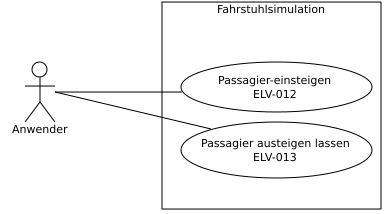
\includegraphics{images/anwenderAWF.png}
	\label{fig:anwenderAWF}
	\caption{Anwendungsfalldiagramm aus Sicht des Anwenders}
\end{figure}

Die Eingangs- und Ausgangsdaten, sowie einige Bemerkungen zu den Anwendungsfällen sind in folgender Tabelle zusammengefasst.

 {
\vspace{1cm}
\hspace{-0,5cm}
\footnotesize
\begin{tabular}{|p{1,5cm}|p{2,5cm}|p{2,5cm}|p{2,5cm}|p{2cm}|}
	\hline
		\textbf{Funktion} &
		\textbf{Eingangsdaten} &
		\textbf{Ausgangsdaten} &
		\textbf{Bemerkungen} &
		\textbf{abstrakter AWD} \\
	\hline \hline
		\textit{Passagier \newline einsteigen} &
		Betätigung der entsprechenden Schaltfläche &
		Visuelle Bestätigung der Eingabe &
		Betreten mehr als 8 Personen den Lift kann eine Überlastsituation auftreten&
		\textbf{Passagier /\newline Monteur\newline steuern} \\
	\cline{1-4}
		\textit{Passagier \newline aussteigen} &
		Betätigung der entsprechenden Schaltfläche &
		Visuelle Bestätigung der Eingabe &
		&
		\\
	\hline
\end{tabular}
}

\section{Anwendungsfälle - Passagiersicht}
Aus dieser Perspektive ergeben sich drei voneinander unabhängige Anwendungsfälle:

\begin{itemize}
	\item \textit{\textbf{Fahrtwunsch - Passagier}} (ELV-011)
	\item \textit{\textbf{Fahrstuhlruf }} (ELV-014)
	\item \textit{\textbf{Fahrtwunsch - Monteur }} (ELV-015)
\end{itemize}


\begin{figure}[hbt]
	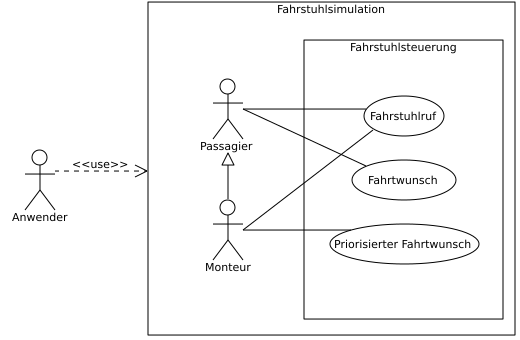
\includegraphics{images/passagierAWF.png}
	\label{fig:passagierAWF}
	\caption{Anwendungsfalldiagramm aus Sicht des Passagieres}
\end{figure}
Beim Monteur handelt es sich um eine Spezialisierte Form eines Passagieres der die Möglichkeit hat einen \glslink{PrioFahrtwunsch}{priorisierten Fahrtwunsch} durchzuführen.
Die Eingangs-, Ausgangsdaten, sowie Bemerkungen sind wiederum in folgender Tabelle zusammengefasst.

 {
\vspace{1cm}
\hspace{-0,5cm}
\footnotesize
\begin{tabular}{|p{2cm}|p{3cm}|p{3cm}|p{3cm}|}
	\hline
		\textbf{Funktion} &
		\textbf{Eingangsdaten} &
		\textbf{Ausgangsdaten} &
		\textbf{Bemerkungen} \\
	\hline \hline
		\textit{Fahrtwunsch \newline Passagier} &
		Etagenwahl (innen) &
		Leuchten der Wunschetage &
		Übergabe des Wunsches an Liftsteuerung \\
	\hline
		\textit{Fahrstuhlruf} &
		Drücken eines der beiden Rufknöpfe (außen) &
		Leuchten der Ruftaste &
		Übergabe des Wunsches an Liftsteuerung  \\
	\hline
		\textit{Fahrtwunsch \newline Monteur} &
		Drücken des Schlüsselsymbols und der Rufetage &
		Leuchten der des Schlüsselsymbols und der Wunschetage &
		Übergabe des Wunsches an Liftsteuerung  \\
	\hline
\end{tabular}
}

\section{Qualitätsanforderungen}
Benutzerfreundlichkeit und die intuitive Bedienbarkeit des Software-Systems haben vor allem im Lehrbetrieb große Wichtigkeit. Aktivitäten des Systems sollten erst nach der Interaktion des Benutzers beginnen und nicht automatisch starten. So ist sicher gestellt, dass der Benutzer in jeder Situation genügend Zeit hat, um das vergangene und zukünftige Verhalten des Systems nachvollziehen und durchdenken zu können. 

\paragraph{}
Weiterhin wird sichergestellt, dass jede Interaktion des Benutzers mit dem System eine Rückmeldung an den Benutzer gibt. Hier werden vor allem Methoden der visuellen Rückmeldung Anwendung finden.

\section{Rahmenbedingungen}

